\subsection{Arquitetura do Sistema}
\label{sec:arquitetura}

Em alto nível, o sistema é composto por três elementos: a \textbf{aplicação cliente}, executada no navegador (e implantada em ambiente de borda); a \textbf{API REST}, que concentra a lógica de domínio; e o \textbf{banco de dados} relacional. O cliente comunica-se com a API exclusivamente via HTTP/JSON, e somente a API acessa o banco. Tanto o servidor quanto o cliente foram estruturados segundo o mesmo princípio --- separação de responsabilidades em camadas com fluxo de dados unidirecional ---, de modo que a arquitetura do cliente \textbf{espelha} a do servidor. A Figura~\ref{fig:arquitetura} sintetiza essa organização em camadas e o sentido único do fluxo de dados, do cliente até o banco; as subseções a seguir descrevem cada lado.

\begin{figure}[H]
\centering
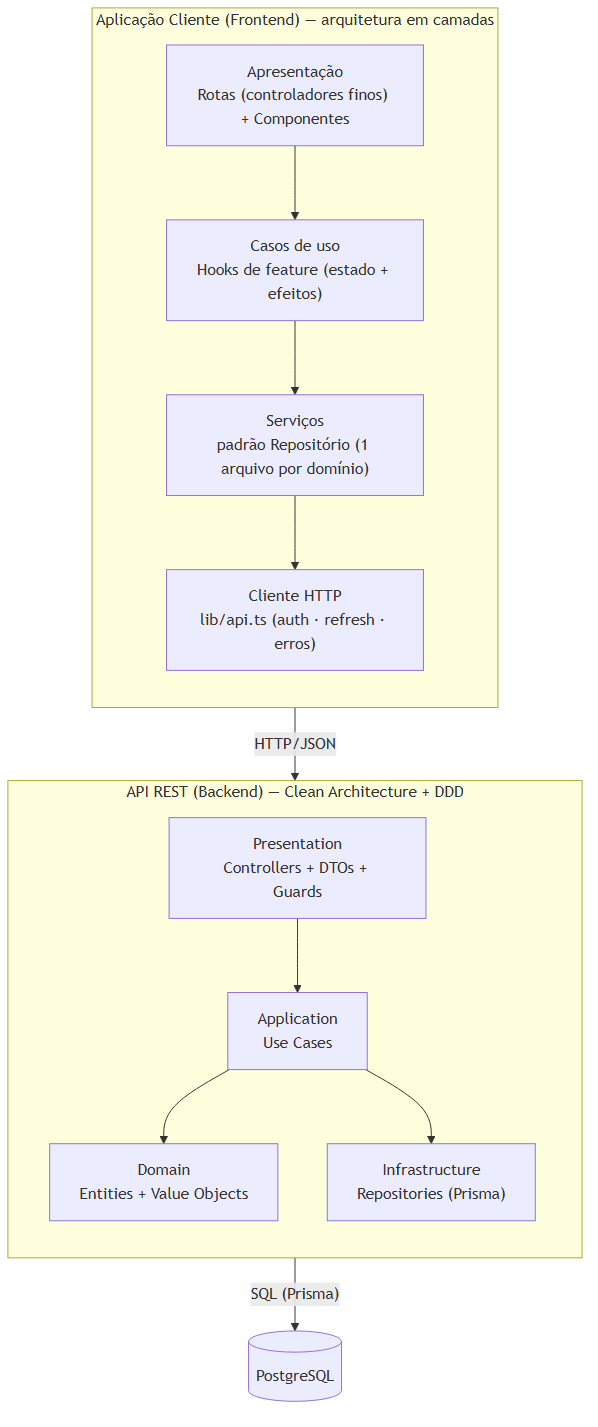
\includegraphics[width=0.6\textwidth]{imagens/arquitetura.png}
\caption{Arquitetura em camadas do sistema --- aplicação cliente, API REST e banco de dados.}
\label{fig:arquitetura}
\end{figure}

\subsubsection{Backend --- Clean Architecture e DDD}

A arquitetura do servidor foi estruturada seguindo os princípios da \textit{Clean Architecture} e do \textit{Domain-Driven Design} (DDD), organizando o sistema em camadas bem definidas que isolam responsabilidades e permitem independência de frameworks externos.

\begin{enumerate}
\item \textbf{Camada de Apresentação (Presentation)}: Controladores REST que orquestram requisições HTTP, validação de DTOs, autenticação JWT e retorno de respostas formatadas.
\begin{itemize}
    \item Controllers: Mapeiam rotas HTTP para casos de uso.
    \item DTOs: Data Transfer Objects com validação via class-validator.
    \item Presenters: Formatam respostas de domínio para o cliente.
    \item Mappers: Convertem entidades de domínio em respostas HTTP.
\end{itemize}

\item \textbf{Camada de Aplicação (Application)}: Orquestra regras de negócio através de Use Cases.
\begin{itemize}
    \item Use Cases: Implementam a lógica de negócio de forma testável e independente.
    \item Aplicação: Coordena fluxo entre domínio e infraestrutura.
    \item Exceptions: Erros de aplicação específicos (ex: \textit{MembershipAlreadyExistsError}).
\end{itemize}

\item \textbf{Camada de Domínio (Domain)}: Contém regras de negócio centrais, completamente independentes de frameworks.
\begin{itemize}
    \item Entities: Objetos com identidade única (ex: User, Organization).
    \item Value Objects: Encapsulam validações de dados (ex: Email, CNPJ, Slug, Money).
    \item Interfaces: Abstraem contratos de repositórios e serviços.
    \item Erros de Domínio: Exceções específicas do negócio.
\end{itemize}

\item \textbf{Camada de Infraestrutura (Infrastructure)}: Implementação de detalhes técnicos.
\begin{itemize}
    \item Repositories: Implementação do padrão Repositório com Prisma.
    \item Database: Configuração do Prisma e conexão com PostgreSQL.
    \item Mappers: Conversão entre entidades de domínio e modelos de persistência.
    \item Providers: Serviços específicos (ex: Bcrypt para hash de senhas).
\end{itemize}

\item \textbf{Camada Compartilhada (Shared)}: Componentes reutilizáveis.
\begin{itemize}
    \item Domain Errors e Value Objects compartilhados.
    \item Guards (JWT authentication, RolesGuard, TenantFilterGuard, DevGuard).
    \item Interceptadores de logging.
    \item Filters de exceção global.
    \item UnitOfWork e DbContext para transações atômicas.
    \item PrismaModule para injeção da conexão em toda a aplicação.
\end{itemize}
\end{enumerate}

Cada módulo de negócio segue a mesma estrutura hierárquica, com um diretório por camada, conforme a Tabela~\ref{tab:modulo_estrutura} (exemplificada com o módulo de usuários).

\begin{table}[H]
\centering
\caption{Estrutura de diretórios de um módulo do \textit{backend} (exemplo: \texttt{user})}
\label{tab:modulo_estrutura}
\begin{tabularx}{\textwidth}{l X}
\toprule
\textbf{Camada (diretório)} & \textbf{Conteúdo típico} \\
\midrule
\texttt{application/}    & DTOs e casos de uso (ex.: \texttt{create-user}, \texttt{find-all-users}, \texttt{find-user-by-id}). \\
\texttt{domain/}         & Entidades, erros de domínio e interfaces de repositório (ex.: \texttt{user.entity}, \texttt{user.errors}, \texttt{user.repository}). \\
\texttt{infrastructure/} & Implementação Prisma do repositório e \textit{mappers} de persistência. \\
\texttt{presentation/}   & Controladores REST e \textit{mappers} de resposta HTTP. \\
\texttt{user.module.ts}  & Declaração do módulo NestJS, que conecta as quatro camadas via injeção de dependência. \\
\bottomrule
\end{tabularx}
\end{table}

Os principais padrões de \textit{design} implementados no servidor são: \textbf{Repositório} (abstração da persistência), \textbf{Injeção de Dependência} (nativa do NestJS), \textbf{Value Objects} (validação de valores complexos), \textbf{Use Cases} (cada operação de negócio como classe testável), \textbf{Guards} (proteção de rotas), \textbf{Interceptadores} (\textit{logging} centralizado), \textbf{Filters de Exceção} (tratamento global de erros), \textbf{Soft Delete} (exclusão por status/\textit{timestamp}) e \textbf{UnitOfWork} (transações atômicas via \texttt{AsyncLocalStorage} sem expor Prisma à camada de aplicação).

\subsubsection{Frontend --- Arquitetura em Camadas}

A arquitetura do cliente espelha a separação do servidor, distribuindo responsabilidades em quatro camadas atravessadas por um fluxo de dados unidirecional, conforme a Figura~\ref{fig:fe_arquitetura}.

\begin{figure}[H]
\centering
\setlength{\fboxsep}{8pt}
\fbox{%
\begin{minipage}{0.88\textwidth}
\centering
\textbf{Apresentação}\\
\texttt{src/routes} + componentes de tela\\
\small rotas finas, composição visual e dados recebidos por propriedades\\[0.2cm]
\(\downarrow\) invocam\\[0.2cm]
\textbf{Hooks de feature}\\
\texttt{src/features/*/hooks}\\
\small casos de uso do cliente: estado, busca, filtros e efeitos\\[0.2cm]
\(\downarrow\) chamam\\[0.2cm]
\textbf{Serviços}\\
\texttt{src/services}\\
\small repositórios de API agrupados por domínio\\[0.2cm]
\(\downarrow\) usam\\[0.2cm]
\textbf{Cliente HTTP}\\
\texttt{src/lib/api.ts}\\
\small autenticação, renovação de sessão e normalização de erros\\[0.2cm]
\(\downarrow\) HTTP/JSON\\[0.2cm]
\textbf{Movy API}
\end{minipage}}
\caption{Arquitetura em camadas da aplicação cliente}
\label{fig:fe_arquitetura}
\end{figure}

A camada de \textbf{apresentação} compõe-se das rotas e dos componentes. As rotas são deliberadamente finas --- controladores enxutos cuja função é instanciar um \textit{hook} de caso de uso e repassar seus dados aos componentes ---, e os componentes recebem dados apenas por propriedades, sem realizar requisições próprias. A camada de \textbf{casos de uso} materializa-se nos \textit{hooks de feature}, que encapsulam a obtenção de dados, o estado associado (carregamento, erro, conteúdo) e os efeitos colaterais de uma operação de domínio. A camada de \textbf{serviços} implementa o padrão Repositório: cada arquivo agrupa as chamadas a um conjunto coeso de \textit{endpoints} e esconde detalhes de transporte. Por fim, o \textbf{cliente HTTP} é o ponto único de comunicação com a API, responsável por anexar credenciais, normalizar erros e renovar a sessão de forma transparente. Por convenção, nenhum componente ou rota chama o cliente HTTP diretamente --- toda comunicação passa por um serviço.

O código organiza-se em \textbf{módulos de feature}: cada domínio reúne, em um único diretório, seus \textit{hooks} e componentes, como sintetiza a Tabela~\ref{tab:fe_estrutura}. Essa estratificação confere ao cliente \textbf{localidade de mudança} (alterações no contrato de um \textit{endpoint} afetam somente o serviço correspondente) e \textbf{coesão por domínio}.

\begin{table}[H]
\centering
\caption{Estrutura de diretórios da aplicação cliente}
\label{tab:fe_estrutura}
\begin{tabularx}{\textwidth}{l X}
\toprule
\textbf{Diretório} & \textbf{Papel} \\
\midrule
\texttt{routes/}     & Rotas \textit{file-based} (TanStack Router) --- controladores finos. \\
\texttt{features/}   & Módulos de domínio (\textit{hooks} + componentes): \texttt{trips}, \texttt{bookings}, \texttt{organizations}, \texttt{drivers}, \texttt{templates}, \texttt{vehicles}, \texttt{scheduling}, \texttt{subscriptions}, \texttt{financial}. \\
\texttt{services/}   & Camada de serviços (padrão Repositório, um arquivo por domínio). \\
\texttt{components/} & Componentes de apresentação: \texttt{ui/} (shadcn), \texttt{layout/}, \texttt{feedback/}, \texttt{visual/}. \\
\texttt{lib/}        & Infraestrutura compartilhada: \texttt{api.ts}, contextos de autenticação e papel, tipos, formatação e \textit{timezone}. \\
\bottomrule
\end{tabularx}
\end{table}

